%%%%%%%%%%%%%%%%%%%%%%%%%%%%%%%%%%%%%%%%%
% Beamer Presentation
% LaTeX Template
% Version 1.0 (10/11/12)
%
% This template has been downloaded from:
% http://www.LaTeXTemplates.com
%
% License:
% CC BY-NC-SA 3.0 (http://creativecommons.org/licenses/by-nc-sa/3.0/)
%
%%%%%%%%%%%%%%%%%%%%%%%%%%%%%%%%%%%%%%%%%

%----------------------------------------------------------------------------------------
%	PACKAGES AND THEMES
%----------------------------------------------------------------------------------------

\documentclass[11pt, xcolor=dvipsnames]{beamer}

\mode<presentation> {

% The Beamer class comes with a number of default slide themes
% which change the colors and layouts of slides. Below this is a list
% of all the themes, uncomment each in turn to see what they look like.

%\usetheme{default}
%\usetheme{AnnArbor}
%\usetheme{Antibes}
%\usetheme{Bergen}
%\usetheme{Berkeley}
%\usetheme{Berlin}
%\usetheme{Boadilla}
%\usetheme{CambridgeUS}
%\usetheme{Copenhagen}
%\usetheme{Darmstadt}
%\usetheme{Dresden}
%\usetheme{Frankfurt}
%\usetheme{Goettingen}
%\usetheme{Hannover}
%\usetheme{Ilmenau}
%\usetheme{JuanLesPins}
%\usetheme{Luebeck}
\usetheme{Madrid}
%\usecolortheme{owl}
%\usetheme{Malmoe}
%\usetheme{Marburg}
%\usetheme{Montpellier}
%\usetheme{PaloAlto}
%\usetheme{Pittsburgh}
%\usetheme{Rochester}
%\usetheme{Singapore}
%\usetheme{Szeged}
%\usetheme{Warsaw}

% As well as themes, the Beamer class has a number of color themes
% for any slide theme. Uncomment each of these in turn to see how it
% changes the colors of your current slide theme.

%\usecolortheme{albatross}
%\usecolortheme{beaver}
%\usecolortheme{beetle}
%\usecolortheme{crane}
%\usecolortheme{dolphin}
%\usecolortheme{dove}
%\usecolortheme{fly}
%\usecolortheme{lily}
%\usecolortheme{orchid}
%\usecolortheme{rose}
\usecolortheme{seagull}
%\usecolortheme{seahorse}


%\setbeamertemplate{footline} % To remove the footer line in all slides uncomment this line
%\setbeamertemplate{footline}[page number] % To replace the footer line in all slides with a simple slide count uncomment this line

%\setbeamertemplate{navigation symbols}{} % To remove the navigation symbols from the bottom of all slides uncomment this line
}
\usepackage[utf8]{inputenc}
\usepackage[english]{babel}

\usepackage{lmodern}
\usepackage{graphicx} % Allows including images
\usepackage{booktabs} % Allows the use of \toprule, \midrule and \bottomrule in tables
\usepackage{mathtools}
\usepackage{lmodern}
\usepackage{xcolor}
\usepackage{scrextend}
\usepackage{tikz}
\usepackage{caption2}
\usepackage{dirtytalk}
\changefontsizes{6pt}
\newcommand{\imagesource}[1]{{\footnotesize $\copyright$ #1}}
%------------------------
----------------------------------------------------------------
%	TITLE PAGE
%----------------------------------------------------------------------------------------

\title{String Theory} % The short title appears at the bottom of every slide, the full title is only on the title page

\author{Nathanael Noir} % Your name
\institute[University of Vienna] % Your institution as it will appear on the bottom of every slide, may be shorthand to save space
{
University of Vienna\\ % Your institution for the title page
\medskip
\textit{john@smith.com} % Your email address
}
\date{\today} % Date, can be changed to a custom date

\begin{document}

\begin{frame}
\titlepage % Print the title page as the first slide
\end{frame}
\begin{frame}
\frametitle{The \(\mathbb{R}^{1}/ \mathbb{Z}_{2}\) Orbifold}
The simplest example of an orbifold is possibly the \alert{\(\mathbb{R}^{1}/\mathbb{Z}_{2}\)} orbifold, where \(\mathbb{R}^{1}\) is the real line as a one-dimensional manifold parametrized by the coordinate \(x\) and \(\mathbb{Z}_{2}\) is an abelian reflection group \(\mathbb{Z}_{2}=\{1,\operatorname{T}\}\) with respect to some axis. The action of \(\mathbb{Z}_{2}\) on \(\mathbb{R}^{1}\) is given by \\
\begin{equation}
	\operatorname{T}: x \mapsto -x 
\end{equation}\\
 After the transformation one can  consider the identification \(x\sim-x\). Strictly speaking and to put it in a more \say{compact} form:
 \begin{equation}
 	x\sim \operatorname{T}(x)
 \end{equation}
  This identification has clearly a fixed point (points that are related to themselves by the identification). The point \(x = 0\) is the unique fixed point of the identification.\\ A fundamental domain can be chosen to be the half-line \(x \geq 0\). The boundary point \(x = 0\) must of course be included in the fundamental domain. The halfline \(x \geq 0\) is called an \(\mathbb{R}^{1}/\mathbb{Z}_{2}\) orbifold. This is the simplest example of an orbifold, a space obtained by identifications that have fixed points (an illustration can be seen in Fig. \ref{fig:2}). If the transformation \(\operatorname{T}\) is applied twice, it gives back the original coordinate.\\\\

\tikzset{every picture/.style={line width=0.75pt}} %set default line width to 0.75pt
\begin{figure}[!h]
\begin{tikzpicture}[x=0.75pt,y=0.75pt,yscale=-1,xscale=1]
%uncomment if require: \path (0,300); %set diagram left start at 0, and has height of 300

%Straight Lines [id:da9478831451585463]
\draw    (58.94,139.54) -- (216.5,139.99) ;
\draw [shift={(219.5,140)}, rotate = 180.16] [fill={rgb, 255:red, 0; green, 0; blue, 0 }  ][line width=0.08]  [draw opacity=0] (10.72,-5.15) -- (0,0) -- (10.72,5.15) -- (7.12,0) -- cycle    ;

%Straight Lines [id:da6345163802859558]
\draw    (134,136) -- (134,144.1) ;


%Curve Lines [id:da09081212715547904]
\draw [color={rgb, 255:red, 208; green, 2; blue, 27 }  ,draw opacity=1 ]   (85.06,121.9) .. controls (86.13,97.49) and (102.17,83.03) .. (121.1,78.53) .. controls (148.68,71.97) and (182.38,86.53) .. (184.87,122.21) ;
\draw [shift={(185,125)}, rotate = 268.65999999999997] [fill={rgb, 255:red, 208; green, 2; blue, 27 }  ,fill opacity=1 ][line width=0.08]  [draw opacity=0] (8.93,-4.29) -- (0,0) -- (8.93,4.29) -- cycle    ;
\draw [shift={(85,125)}, rotate = 269.55] [fill={rgb, 255:red, 208; green, 2; blue, 27 }  ,fill opacity=1 ][line width=0.08]  [draw opacity=0] (8.93,-4.29) -- (0,0) -- (8.93,4.29) -- cycle    ;
%Straight Lines [id:da6458003311005677]
\draw    (360.5,144) -- (360,134) ;


%Straight Lines [id:da9217466899809739]
\draw    (439.5,139) -- (361,139) ;

\draw [shift={(442.5,139)}, rotate = 180] [fill={rgb, 255:red, 0; green, 0; blue, 0 }  ][line width=0.08]  [draw opacity=0] (10.72,-5.15) -- (0,0) -- (10.72,5.15) -- (7.12,0) -- cycle    ;
%Straight Lines [id:da15119105433695323]
\draw  [dash pattern={on 4.5pt off 4.5pt}]  (361,139) -- (286.5,139) ;
% Text Node
\draw (211,154) node    {$x$};
% Text Node
\draw (136,155) node    {$0$};
% Text Node
\draw (441,154) node    {$x$};
% Text Node
\draw (360,156) node    {$0$};
\end{tikzpicture}
\centering
\caption{The identification \(x \slim -x\) on the real line \(\mathbb{R}^{1}\) yields the half-line. This is the \(\mathbb{R}^{1}/ \mathbb{Z}_{2}\) orbifold.}
\label{fig:2}
\end{figure}

\end{frame}
\begin{frame}
\frametitle{Why are Orbifolds Interesting and Useful in Physics?}
\alert{Orbifolds} are roughly speaking pretty elegant spaces with curvature singularities. In classical general relativity or quantum mechanics it is fairly difficult to treat such manifolds with singularities correctly. Just imagine doing GR on the geometry of a cone. The curvature of the cone is flat everywhere, except at the tip, where the curvature is singular.\\
String theory on the other hand is capable of handling these \say{naked} singularities. It can further be shown, that GR is a low energy limit of string theory. In the low energy description the singular geometry can be smoothed out. This procedure is called \alert{resolving a singularity}.\\ Orbifolds are further very interesting in physics because configuration and phase spaces of gauge systems are orbifolds after the removal of the gauge redundancy.\\\\  
\tikzset{every picture/.style={line width=0.75pt}} %set default line width to 0.75pt
\begin{figure}[!h]
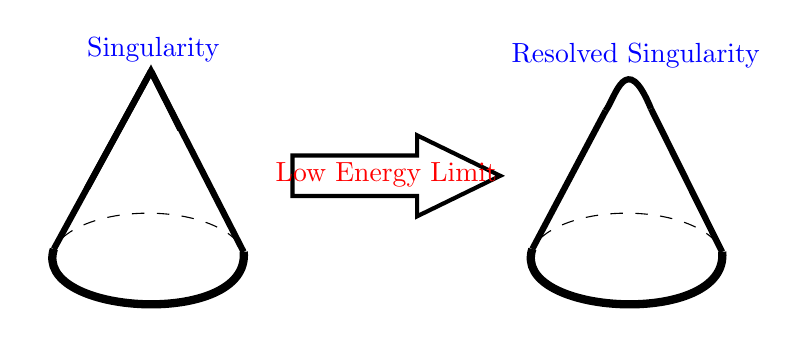
\begin{tikzpicture}[x=0.65pt,y=0.75pt,yscale=-0.5,xscale=0.7]
%uncomment if require: \path (0,431); %set diagram left start at 0, and has height of 431

%Shape: Ellipse [id:dp9459243482302933]
\draw  [dash pattern={on 4.5pt off 4.5pt}] (73,290.5) .. controls (73,265.92) and (107.36,246) .. (149.75,246) .. controls (192.14,246) and (226.5,265.92) .. (226.5,290.5) .. controls (226.5,315.08) and (192.14,335) .. (149.75,335) .. controls (107.36,335) and (73,315.08) .. (73,290.5) -- cycle ;
%Straight Lines [id:da40458722770489497]
\draw [line width=2.25]    (75,280.5) -- (152.18,108.95) ;


%Straight Lines [id:da0683426623601252]
\draw [line width=2.25]    (225.69,283.27) -- (152.1,109.11) ;


%Curve Lines [id:da3114600765309612]
\draw [line width=3]    (75,280.5) .. controls (57.5,345) and (231.5,357) .. (225.77,283.1) ;


%Shape: Right Angle [id:dp3627650174644287]
\draw  [line width=2.25]  (101.36,222.03) -- (152.1,109.11) -- (175.43,165.37) ;
%Shape: Ellipse [id:dp2926192456965184]
\draw  [dash pattern={on 4.5pt off 4.5pt}] (453,290.5) .. controls (453,265.92) and (487.36,246) .. (529.75,246) .. controls (572.14,246) and (606.5,265.92) .. (606.5,290.5) .. controls (606.5,315.08) and (572.14,335) .. (529.75,335) .. controls (487.36,335) and (453,315.08) .. (453,290.5) -- cycle ;
%Straight Lines [id:da2506665033019121]
\draw [line width=2.25]    (455,280.5) -- (513.19,147.3) ;


%Straight Lines [id:da6044413488669527]
\draw [line width=2.25]    (605.69,283.27) -- (549.19,145.3) ;


%Curve Lines [id:da18617884171476418]
\draw [line width=3]    (455,280.5) .. controls (437.5,345) and (611.5,357) .. (605.77,283.1) ;


%Curve Lines [id:da4356951242193631]
\draw [line width=2.25]    (513.19,147.3) .. controls (521.05,134.69) and (529.5,87) .. (549.19,145.3) ;


%Right Arrow [id:dp8956775508702847]
\draw  [line width=1.5]  (264.5,190.5) -- (363.5,190.5) -- (363.5,171) -- (429.5,210) -- (363.5,249) -- (363.5,229.5) -- (264.5,229.5) -- cycle ;

% Text Node
\draw (154,88) node   [align=left] {\textcolor{Blue}{Singularity}};
% Text Node
\draw (537,94) node   [align=left] {\textcolor{Blue}{Resolved Singularity}};
% Text Node
\draw (339,209) node   [align=left] {\textcolor{Red}{Low Energy Limit}};


\end{tikzpicture}
\centering
\caption{The low energy limit of string theory is a field theory, which contains GR in it. In the low energy description String theory on the cone resolves the singulariy. The so-called twisted sector states smooth out the singularity.}
\label{fig:1}
\end{figure}

\end{frame}
\begin{frame}
\frametitle{explanation}




%\begin{columns}
%\begin{column}{0.5\textwidth}
\alert{Pickover's superfactorial} is defined by
\begin{equation}
	\boxed{
    n\$\equiv{^{n!}\left(n!\right)}}
\end{equation}

where the \alert{hyper-4-operation} (tetration) is defined recursively as
\begin{equation}
{^{n}a}:=\left\{\begin{array}{ll}
{1} & {\text { if } n=0} \\
{a^{(n-1) a}} & {\text { if } n>0}
\end{array}\right.
\end{equation}
%\end{column}
%\begin{column}{0.5\textwidth}  
%    \begin{center}
%     Example: 
%     \begin{equation}
%     	3\$=
%6^{6^{6^{6^{6^{6}}}}}
%     \end{equation}
%     \end{center}
%\end{column}
%\end{columns}
\end{frame}

\begin{frame}
\frametitle{The Lagrangian for Quantum Chromodynamics}
The Lagrangian for Quantum Chromodynamics is
\begin{equation}
\begin{split}
\mathcal{L}_{\textcolor{Red}{Q}\textcolor{Blue}{C}\textcolor{OliveGreen}{D}} &=\sum_{i=1}^{6}\left[\hbar c \bar{\Psi}_{i} \gamma^{\mu} D_{\mu} \Psi_{i}+m_{i} c^{2} \bar{\Psi}_{i} \Psi_{i}\right]+\frac{1}{16 \pi}\left(\partial_{\mu} A_{\nu}^{a}-\partial_{\nu} A_{\mu}^{a}\right)\left(\partial^{\mu} A^{\nu a}-\partial^{\nu} A^{\mu a}\right) \\
&-\frac{g}{16 \pi} f^{a d e} A_{\mu}^{d} A_{\nu}^{e}\left(\partial^{\mu} A^{\nu a}-\partial^{\nu} A^{\mu a}\right)-\frac{g}{16 \pi} f^{a b c} A^{\mu b} A^{\nu c}\left(\partial_{\mu} A_{\nu}^{a}-\partial_{\nu} A_{\mu}^{a}\right) \\
&+\frac{g^{2}}{16 \pi} f^{a b c} f^{a d e} A_{\mu}^{b} A_{\nu}^{c} A^{\mu d} A^{\nu e}
\end{split}
\end{equation}
where \(D_{\mu} \Psi=\partial_{\mu}+i g \lambda \cdot A_{\mu} \Psi\) with the eight generators \(\lambda\) of \(\mathrm{SU}(3)\) and the sum goes over all six flavors of quarks. The Dirac Lagrangian handles quarks and antiquarks such that the antiquarks do not have to be listed separately. Each \(\Psi_{i}\) is a vector in color space with the three components \(\textcolor{Red}{\Psi_{r i}}, \textcolor{Blue}{\Psi_{b i}}, \textcolor{OliveGreen}{\Psi_{g_{i}}},\) and the three colors \((\textcolor{Red}{r}, \textcolor{Blue}{b}, \textcolor{OliveGreen}{g})\) play the role of charges and interactions via eight gluons.
\begin{itemize}
	\item This and the non-abelian character of \(\mathrm{SU}(3)\) makes it already more complicated than Quantum Electrodynamics with one type of charge instead of three and one photon instead of eight gluons.
	\item Another complication comes from the fact that Quantum Chromodynamics is defined in terms of quarks, but one can only observe and experiment the bound states which are hadrons.
\end{itemize}


The first line of the Lagrangian looks similar to the case for Quantum Electrodynamics, but the second and third line of the Lagrangian come in addition representing the gluon-gluon interactions. Therefore there will be Feynman diagrams with \alert{pure gluon vertices}.\\ The two terms in the second line lead to vertices with three gluons and the term in the third line results in vertices with four gluons.
\end{frame}


\begin{frame}
\frametitle{d-dimensional solid angle}
	\(\mathrm{d} \Omega_{d}\) is the differential solid angle of the \(d\)-dimensional unit sphere
	\begin{equation}
		\(\Omega_{d}=\sin ^{d-2}\left(\varphi_{d-1}\right) \sin ^{d-3}\left(\varphi_{d-2}\right) \ldots \sin \left(\varphi_{2}\right) \mathrm{d} \varphi_{1} \ldots \mathrm{d} \varphi_{d-1}\)
	\end{equation}
with \(\varphi_{i}\) denoting the angle relative to the \(i\)-th axis and \(0 \leq \varphi_{1}<2 \pi, 0 \leq \varphi_{i}<\pi\) for \(i>1\) (you can check that this produces the correct results in 2 and 3 dimensions). The expression for the full solid angle \(\Omega_{d}=\int \mathrm{d} \Omega_{d}\) can be derived with the exponential function trick:
\begin{equation}
	\begin{aligned}
(\sqrt{\pi})^{d} &=\left(\int \mathrm{d} x e^{-x^{2}}\right)^{d}=\prod_{i=1}^{d} \int_{-\infty}^{\infty} \mathrm{d} x_{i} e^{-x_{i}^{2}}=\left(\prod_{i=1}^{d} \int_{-\infty}^{\infty} \mathrm{d} x_{i}\right) e^{-\sum_{j=1}^{d} x_{j}^{2}} \\
&=\int \mathrm{d} \Omega_{d} \int \mathrm{d} r r^{d-1} e^{-r^{2}}=\Omega_{d} \frac{1}{2} \Gamma\left(\frac{d}{2}\right) \\
\end{aligned}
\end{equation}

\begin{equation}
\begin{centering}
		\boxed{\Omega_{d}=& \frac{2 \pi^{d / 2}}{\Gamma\left(\frac{d}{2}\right)}}
\end{centering}
\end{equation}
\(\left.\Gamma \text { is the \alert{gamma function} (with } \Gamma(1+z)=z \Gamma(z), \Gamma(1)=1, \Gamma\left(\frac{1}{2}\right)=\sqrt{\pi}, \ldots)\) and we used \alert{Euler's integral form} (after a substitution \(\left.t=r^{2})\)
\begin{equation}
	\(\Gamma(z)=\int_{0}^{\infty} \mathrm{d} t e^{-t} t^{z-1}\),\;\;\;
\((\operatorname{Re}(z)>0)\)
\end{equation}

\end{frame}
\begin{frame}
\frametitle{Overview} % Table of contents slide, comment this block out to remove it
\tableofcontents % Throughout your presentation, if you choose to use \section{} and \subsection{} commands, these will automatically be printed on this slide as an overview of your presentation
\end{frame}

%----------------------------------------------------------------------------------------
%	PRESENTATION SLIDES
%----------------------------------------------------------------------------------------

\begin{frame}
\frametitle{d-dimensional solid angle}

\tikzset{every picture/.style={line width=0.75pt}} %set default line width to 0.75pt        
\begin{figure}[!h]
\centering
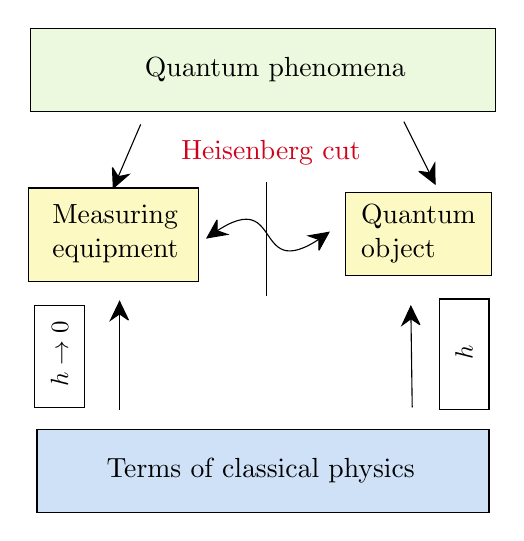
\begin{tikzpicture}
[x=0.75pt,y=0.75pt,yscale=-1,xscale=1]
%uncomment if require: \path (0,346); %set diagram left start at 0, and has height of 346

\draw  [fill={rgb, 255:red, 248; green, 231; blue, 28 }  ,fill opacity=0.27 ]  (237, 110) rectangle (319, 155)   ;
\draw  [fill={rgb, 255:red, 248; green, 231; blue, 28 }  ,fill opacity=0.27 ]  (390, 112) rectangle (460, 152)   ;
\draw  [fill={rgb, 255:red, 74; green, 144; blue, 226 }  ,fill opacity=0.27 ]  (241.23, 226.33) rectangle (459, 266.33)   ;
\draw    (281,217) -- (281,164.67) ;
\draw [shift={(281,164.67)}, rotate = 450] [color={rgb, 255:red, 0; green, 0; blue, 0 }  ][fill={rgb, 255:red, 0; green, 0; blue, 0 }  ]  (8.93,-4.29) -- (0,0) -- (8.93,4.29) -- (5.93,0) -- (8.93,-4.29)    ;

\draw    (422,215.67) -- (421.33,167) ;
\draw [shift={(421.33,167)}, rotate = 449.22] [color={rgb, 255:red, 0; green, 0; blue, 0 }  ][fill={rgb, 255:red, 0; green, 0; blue, 0 }  ]  (8.93,-4.29) -- (0,0) -- (8.93,4.29) -- (5.93,0) -- (8.93,-4.29)    ;

\draw  [fill={rgb, 255:red, 184; green, 233; blue, 134 }  ,fill opacity=0.27 ]  (237.9, 33) rectangle (462, 73)   ;
\draw    (323.17,134) .. controls (363.17,104) and (341.83,161.33) .. (381.83,131.33) ;
\draw [shift={(381.83,131.33)}, rotate = 504.52] [color={rgb, 255:red, 0; green, 0; blue, 0 }  ][fill={rgb, 255:red, 0; green, 0; blue, 0 }  ]  (8.93,-4.29) -- (0,0) -- (8.93,4.29) -- (5.93,0) -- (8.93,-4.29)    ;
\draw [shift={(323.17,134)}, rotate = 324.73] [color={rgb, 255:red, 0; green, 0; blue, 0 }  ][fill={rgb, 255:red, 0; green, 0; blue, 0 }  ]  (8.93,-4.29) -- (0,0) -- (8.93,4.29) -- (5.93,0) -- (8.93,-4.29)    ;
\draw    (418,78) -- (433,108) ;
\draw [shift={(433,108)}, rotate = 243.43] [color={rgb, 255:red, 0; green, 0; blue, 0 }  ][fill={rgb, 255:red, 0; green, 0; blue, 0 }  ]  (8.93,-4.29) -- (0,0) -- (8.93,4.29) -- (5.93,0) -- (8.93,-4.29)    ;

\draw    (291.17,79.33) -- (278,110) ;
\draw [shift={(278,110)}, rotate = 293.24] [color={rgb, 255:red, 0; green, 0; blue, 0 }  ][fill={rgb, 255:red, 0; green, 0; blue, 0 }  ]  (8.93,-4.29) -- (0,0) -- (8.93,4.29) -- (5.93,0) -- (8.93,-4.29)    ;

\draw    (352,107) -- (352,162) ;



\draw (356,53) node  [align=left] {Quantum phenomena};
\draw (279,132) node  [align=left] {Measuring\\equipment};
\draw (425,132) node  [align=left] {Quantum\\object};
\draw (349,246) node  [align=left] {Terms of classical physics};
\draw (354,93) node [color={rgb, 255:red, 208; green, 2; blue, 27 }  ,opacity=1 ] [align=left] {Heisenberg cut};
\draw     (240, 166.42) rectangle (264, 215.75)   ;
\draw (252,190) node [scale=0.9,rotate=-270]  {$h\rightarrow 0$};
\draw     (435, 163.44) rectangle (459, 216.5)   ;
\draw (447,189) node [scale=0.9,rotate=-270]  {$h$};


\end{tikzpicture}

\caption[The Correspondence Principle of QM and the Heisenberg Cut]{The correspondence principle of QM and the Heisenberg Cut.}

\imagesource{Nathanael Noir}
\end{figure}
\end{frame}


%------------------------------------------
\begin{frame}
\frametitle{3 Definitions of Energy-Momentum Tensor}
\begin{block}{Canonical Energy-Momentum Tensor \(\Theta_{\nu}^{\mu}(x)\)}
	Noether's theorem implies that there is a conserved current associated with translations through space and time.
	\begin{equation}
\Theta_{\nu}^{\mu}=\frac{\partial \mathcal{L}(x)}{\partial\left(\partial_{\mu} \phi_{n}\right)} \frac{\partial \phi_{n}(x)}{\partial x^{\nu}}-\delta_{\nu}^{\mu} \mathcal{L}(x).
\end{equation}
	   In the presence of spin the canonical energy-momentum tensor fails to be symmetric. It's also not necessary gauge invariant.
\end{block}
\begin{alertblock}{Hilbert Energy-Momentum Tensor \(T_{\mu}_{\nu}(x)\)}
The Hilbert energy-momentum is defined as follows:
\begin{equation}
T_{\mu}_{\nu}=\frac{-2}{\sqrt{-g}} \frac{\partial\left(\sqrt{-g} \mathcal{L}_{\text {matter }}\right)}{\partial g^{\mu \nu}}.
\end{equation}
where \(\mathcal{L}_{\text {matter }}\) is the non-gravitational part of the Lagrangian density. This tensor is symmetric and gauge-invariant.
\end{alertblock}
\begin{exampleblock}{Belinfante-Rosenfeld \(\theta^{\mu \nu}(x)\)}
	 The Belinfante-Rosenfeld stress energy tensor is constructed from the canonical stress-energy tensor and the spin current in such a way as to be symmetric and still conserved. 
	 \begin{equation}
\theta^{\mu \nu}=\Theta^{\mu \nu}+\partial_{\alpha} f^{\alpha \mu \nu}.
\end{equation}
	 In general relativity, this tensor agrees with the Hilbert energy-momentum tensor.
\end{exampleblock}
\end{frame}

%-------------------------------------------


\begin{frame}
\frametitle{A very simple calculation with an arbitrarily exponentiated differential operator}

%\begin{columns}
%\begin{column}{0.5\textwidth}
For the differential operator $D:=\frac{d}{dx}$ it is generally not intuitively possible to write down an expression for $D^{\alpha}(f(x))$ with arbitrary $\alpha \in \mathbb{C}$ and a sufficiently differentiable function $f(x)$ with $x\in \mathbb{R}$. Here, I make an interesting Ansatz with respect to the spectrum $\Omega (D)$ of $D$. The Eigenfunctions of $D$ are given by functions $g(x) = g_0\cdot\text{exp}\left[\lambda (x-x_0)\right]$ with corresponding Eigenvalue $\lambda$. Therefore the spectrum of $D$ with respect to those Eigenfunctions is given by $\Omega (D) = \mathbb{C}$. Assume the function $f(x)$ can be expressed in terms of a fourier series as follows: $f(x) =\sum_{n\in \mathbb{Z}\setminus \lbrace 0 \rbrace} c_n e^{ i nx} $. Then
\begin{equation}
  D^{\alpha} (f(x)) = \sum_{n\in \mathbb{Z}\setminus \lbrace 0 \rbrace} c_n D^{\alpha} (e^{ i nx}) 
\end{equation}
For a correct choice of a branch of the logarithm it can now be found that for $n\neq 0$
\begin{equation}
    D^{\alpha} (e^{i nx}) =  ( i n)^{\alpha} e^{ i nx} 
\end{equation}
%... e^{\alpha ln(D)} (e^{2\pi i nx}) = e^{\alpha ln(2\pi i n)} (e^{2\pi i nx}) = ... seems actually redundant, due to f(D)=f(\lambda)
(this also holds true for $\alpha =0$) and thus
\begin{equation}
    \boxed{D^{\alpha} (f(x)) = \sum_{n\in \mathbb{Z}\setminus \lbrace 0\rbrace} c_n ( i n)^{\alpha} e^{ i nx} = i^{\alpha}\sum_{n\in \mathbb{Z}\setminus \lbrace 0\rbrace} c_n n^{\alpha} e^{ i nx}}
\end{equation}
In order to know whether or not $D^{\alpha} (f(x))$ exists one would need to check convergence of the series, which is not a given because the differential operator changes its coefficients by a factor $n^{\alpha}$.
%It is not easy to determine $\tilde{c}_0 := \frac{1}{(2\pi i)^{\alpha}}D^{\alpha}(c_0)$. For $c_0=0$, clearly $D^{\alpha} (0) = 0$ if we view $D^{\alpha}$ as a differential operator. For $c_0\neq 0$ an Ansatz can be made as follows:\\
%\mathbcal{Re}(\alpha ) > 0 \Rightarrow \tilde{c}_0 = 0\\
%\mathbcal{Re}(\alpha ) < 0 \\
%\left( \alpha = i\beta \right)\wedge \left(\beta > 0\right)\\
%\left( \alpha = i\beta \right)\wedge \left(\beta < 0\right)
%\end{eqnarray}

\end{frame}
\setbeamercolor{background canvas}{bg=black!100}
\color{white}
\begin{frame}
\frametitle{Fun with Integration}
\begin{eqnarray}
\boxed{\int_0^1 x^{-x} \,dx} = \int_0^1 e^{-x\text{ln}(x)} \,dx = \int_0^1 \sum_{n=0}^{\infty} \frac{(-1)^n x^n (\text{ln}(x))^n}{n!}  =\Box\\
\end{eqnarray}

Now we substitute to simplify the integrand with \(y=-\ln{x}\)
\begin{equation*}
\Box =\int_{\infty}^0 \sum_{n=0}^{\infty} \frac{(-1)^{2n+1} e^{-y(n+1)} y^n}{n!} \, dy= \Delta
\end{equation*}
Yet another substitution \( p=(n+1)y\) yields the following:\\
\begin{equation*}
\begin{split}
\Delta &= \int_{\infty}^0 \sum_{n=0}^{\infty} \frac{(-1) e^{-p} p^n}{n! (n+1)^{n+1}} \, dp =  \sum_{n=0}^{\infty} \int_{\infty}^0 \frac{(-1) e^{-p} p^n}{n! (n+1)^{n+1}} \, dp  \\
&=\sum_{n=0}^{\infty} \frac{1}{n! (n+1)^{n+1}}\int^{\infty}_0  e^{-p} p^n \, dp = \sum_{n=0}^{\infty} \frac{\Gamma (n+1)}{n! (n+1)^{n+1}} \\
&=\sum_{k=1}^{\infty} \frac{1}{k^k} =
\boxed{\sum_{k=1}^{\infty} k^{-k}}
\end{split}
\end{equation*}
\end{frame}


\begin{frame}{Using symmetries to find sums}
Assume the infinite sum $s(t) = \sum_{k=1}^{\infty} (tk)^{-k}$. We want to use its symmetry when transforming $t\rightarrow 1/t$ to deduce an unexpected relation. In order to do so, we first have to find a function that represents this sum. $s(t)$ is differentiable on the set $(0, \infty )$ so we use this to make an Ansatz:
\begin{equation}
\frac{\partial s(t)}{\partial t} = \sum_{k=1}^{\infty}(-k) t^{-k-1}  k^{-k} = \frac{-1}{t^2} \sum_{k=1}^{\infty} (tk)^{-k+1} = \frac{-1}{t^2}\left[ 1+s(t)\right]
\end{equation}
The solution to this differential equation is given by
\begin{equation}
    s(t) = C\;e^{1/t} - 1
\end{equation}
for some arbitrary real constant $C$. It is very hard to find this constant, which is why this will be something to be solved at a later point in time. In general, we would have to evaluate $C = e^{-1/t} + e^{-1/t} s(t)$.
Now, looking at $s(1/t)$, we immediately find that also $c = e^{-t} + e^{-t} s(1/t)$. Clearly these two results for $C$ must be similar, because $s(1) = s(1/1)$. So we find
\begin{equation}
    e^{-1/t} + e^{-1/t} s(t) = e^{-t} + e^{-t} s(1/t)
\end{equation}
which results in
\\
\begin{equation}
    \sum_{k=1}^{\infty} k^{-k} \left[ t^{-k}e^{-1/t} - t^ke^{-t}\right] = e^{-t} - e^{-1/t}
\end{equation}
\\
    $\forall t\in (0,\infty )$
    
\end{frame}


\begin{frame}{Calculating the constant c}
Previously we found $\int_0^1 x^{-x} \,dx = \sum_{k=1}^{\infty} k^{-k}$. This can be used to calculate the constant $c$ as follows
\begin{equation}
    c = \frac{1+\int_0^1 x^{-x} \,dx}{e}
\end{equation}
    in order to find
    \begin{equation}
        s(t) = \sum_{k=1}^{\infty} (tk)^{-k} = \frac{1+\int_0^1 x^{-x} \,dx}{e} \cdot e^{1/t} - 1
    \end{equation}
This means that we have completely determined the sum $s(t)$ up to solving the integral. The problem with this is that the integral can only be solved numerically, unless the sum over $k^{-k}$ itself is evaluated. In order to analytically find a solution for $c$, we still need to evaluate $C = e^{-1/t} + e^{-1/t} s(t)$. Luckily, because $c$ is constant, we know that this equation holds for all $t\in (0,\infty )$. Thus another approach would be to find
\begin{equation}
    c = \lim_{t\rightarrow \infty}\left( e^{-t} + e^{-t} s(1/t)\right) = \lim_{t\rightarrow \infty}\left( e^{-t} s(1/t)\right) =\lim_{t\rightarrow \infty}\left( \frac{s(1/t)}{e^t}\right)
\end{equation}
Even though L'Hopital's rule applies to this limit, it unfortunately doesn't yield a result. This limit is very hard to calculate and unfortunately I haven't found a solution for it up to now...    
\end{frame}
\begin{frame}{The Lausch-constant}
    \begin{equation}
       \boxed{ s(t) = \sum_{k=1}^{\infty} (tk)^{-k} = \ell_0 \cdot e^{1/t} - 1}
    \end{equation}
    $\forall t \in (0, \infty )$. Here $\ell_0$ is the \textbb{Lausch-constant}, which is given by 
    \begin{equation}
        \boxed{\ell_0 = \frac{1+\int_0^1 x^{-x} \,dx}{e}}
    \end{equation}
\end{frame}
\end{document} 